\documentclass[xcolor=dvipsnames]{beamer}
\usepackage[utf8]{inputenc}
\usepackage{hyperref}
\usepackage[super]{nth} % for 1st, 2nd, etc...
\setbeamertemplate{caption}[numbered] %for figures numbering
\usepackage[export]{adjustbox} %for left and right
\usepackage{siunitx} % for degree symbol

\usetheme{CambridgeUS}

\definecolor{UBCblue}{rgb}{0.04706, 0.13725, 0.26667} % UBC Blue (primary)
\definecolor{UBCgrey}{rgb}{0, 0.46, 0.7} % UBC Grey (secondary)

\setbeamercolor{title}{bg=UBCblue,fg=white}
\setbeamercolor{frametitle}{bg=UBCblue, fg=white}
\setbeamercolor{palette primary}{bg=UBCblue,fg=white} %basso a destra
\setbeamercolor{palette secondary}{fg=UBCblue} %basso al centro
\setbeamercolor{palette tertiary}{bg=UBCgrey,fg=white} %basso e alto a sx 

\setbeamercolor{structure}{fg=UBCblue} % itemize, enumerate, etc
\setbeamercolor{section in toc}{fg=UBCblue} % TOC sections
\setbeamercolor{block title}{bg=UBCgrey!50,fg=black}
\setbeamercolor{block title example}{bg=UBCgrey!50,fg=black}

%------------------------------------------------------------
%This block of code defines the information to appear in the
%Title page
\title[Emotion Patterns in Music Playlists] %optional
{Emotion Patterns in Music Playlists}

%\subtitle{\nth{1} meeting}

\author[Sara, Mario] % (optional)
{Sara Giammusso\inst{1}\inst{2} \and Mario Guerriero \inst{1}\inst{2}}

\institute[EURECOM] % (optional)
{
 \inst{1}
 MSc student in Data Science Department, EURECOM, T\'el\'ecom ParisTech, France\\
  \inst{2}%
 MSc student in Department of Control and Computer Engineering, Politecnico di Torino, Italy
}


\date[2018 April 5] % (optional)
{Third Project meeting}


%End of title page configuration block
%-----------------------------------------------------------



%------------------------------------------------------------
%The next block of commands puts the table of contents at the 
%beginning of each section and highlights the current section:

\AtBeginSection[]
{
  \begin{frame}
    \frametitle{Table of Contents}
    \tableofcontents[currentsection]
  \end{frame}
}
%------------------------------------------------------------


\begin{document}

%The next statement creates the title page.
\frame{\titlepage}

%---------------------------------------------------------
%This block of code is for the table of contents after
%the title page
\begin{frame}
\frametitle{Table of Contents}
\tableofcontents
\end{frame}
%---------------------------------------------------------

\section{Introduction}
%Intoduction
\begin{frame}{Introduction}
\begin{block}{Previously On Sara\&Mario Project...}
We analyzed already existent systems and we came up with some decisions about what to do.\\
\end{block}
Next steps:
\begin{itemize}
\item Start building some simple classifiers
\item Evaluate those simple classifiers
\item See how we could improve it
\end{itemize}
\end{frame}

%Model Description
\section{LyricsKMeans: Model Description}

\begin{frame}{The Idea}
\begin{itemize}
\item Based on the same idea of the Nearest Neighbour
\item Find the "closest" song and get its label
\item We are not actually comparing lyrics to each other
\item We compare lyrics we want to classify to 4 points
\begin{itemize}
\item Each point is supposed to be representative of an emotion
\end{itemize}
\end{itemize}
\end{frame}

\begin{frame}{Why 4 points?}
\begin{itemize}
\item Simplicity
\item Speed
\item We just wanted to get some quick insights
\end{itemize}
\end{frame}

\begin{frame}{How it works}
\begin{itemize}
\item Evaluate the word vector norm for each lyrics
\item Group (compute average) lyrics by emotion
\item Given a lyric find the closest representative point
\end{itemize}
\end{frame}

%Model Evaluation
\section{LyricsKMeans: Model Evaluation}

\begin{frame}{1-fold validation}
We used the simplest validation technique: 1-fold validation
\begin{itemize}
\item 90\% for training
\item 10\% for validation
\end{itemize}
\end{frame}

\begin{frame}{Accuracy}
\begin{columns}
\column{0.5\textwidth}
\begin{itemize}
\item Not very impressive
\item Around 28\% accuracy
\end{itemize}
\column{0.5\textwidth}
\begin{figure}
	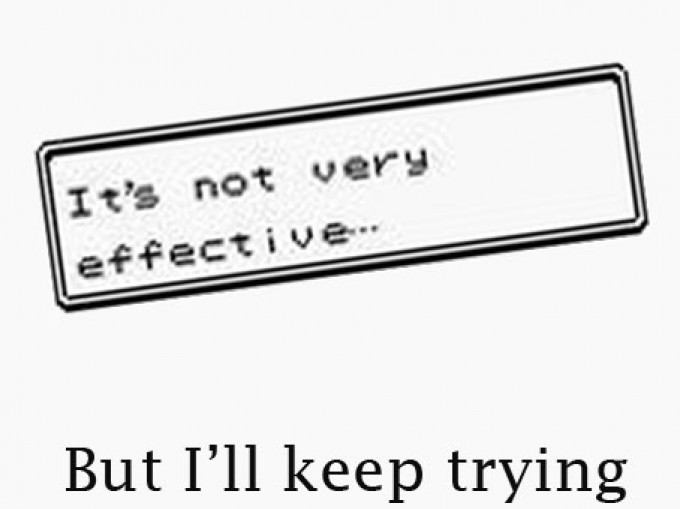
\includegraphics[scale=0.25,left]{./images/not-effective.jpg}
\end{figure}
\end{columns}
\end{frame}

%Model Description
\section{LyricsNN: Model Description}

\begin{frame}{The Idea}
\begin{block}{DISCLAIMER}
This model is slower then the previous one
\end{block}
\begin{itemize}
\item A more general version of the LyricsAverageNN classifier
\item Based on the same idea of the k-Nearest Neighbour (again)
\item Find the "closest" song and get its label
\item Now we are comparing lyrics to each other
\end{itemize}
\end{frame}

\begin{frame}{How it works}
\begin{itemize}
\item Evaluate the word vector norm for each lyrics
\item Do NOT group anything
\item Given a lyric find the closest lyrics and get their majority label
\end{itemize}
\end{frame}

%Model Evaluation
\section{LyricsNN: Model Evaluation}

\begin{frame}{1-fold validation}
We used the same validation technique we used for the previous model
\begin{itemize}
\item 90\% for training
\item 10\% for validation
\end{itemize}
\end{frame}

\begin{frame}{Accuracy}
\begin{columns}
\column{0.5\textwidth}
\begin{itemize}
\item Not very impressive
\item 33\% accuracy (k=1)
\item 30\% accuracy (k=3)
\item 29\% accuracy (k=5)
\end{itemize}
\column{0.5\textwidth}
\begin{figure}
	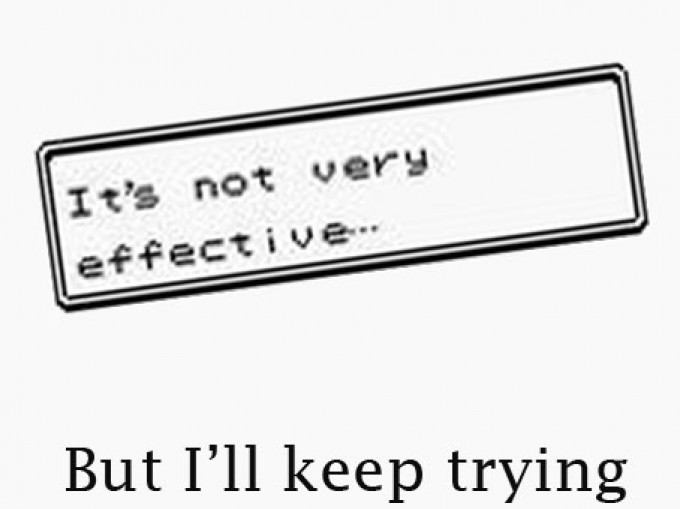
\includegraphics[scale=0.25,left]{./images/not-effective.jpg}
\end{figure}
\end{columns}
\end{frame}


%Conclusions
\section{Conclusion}

\begin{frame}{What's next?}
\begin{itemize}
\item We didn't use Fastext word vectors for the sake of time...
\item We need better feature engineering
\item Move to better classifiers (it didn't make sense to use them for now)
\item Find out some better pre-processing techniques
\item Implement better validation technique (cross-validation!!!)
\end{itemize}
\end{frame}

%References

\section{References}
\begin{frame}[allowframebreaks]{References}
\setbeamertemplate{bibliography item}[text]
 \begin{thebibliography}{99} % Beamer does not support BibTeX so references must be nserted manually as below
\bibitem{p1} spaCy: Industrial-Strength Natural Language Processing
\footnotesize \url{https://spacy.io/}

\bibitem{p8} Intro to NLP with SpaCy
\footnotesize\url{https://nicschrading.com/project/Intro-to-NLP-with-spaCy/}

\end{thebibliography}

\end{frame}

%---------------------------------------------------------

\end{document}
